\chapter{A general overview of the Germanic languages}

This chapter provides an overview of general facts about the Germanic languages. It derives from
slides for teaching courses about Germanic languages that were used by Ekkehard König and passed on
to Matthias Hüning and via Matthias to me, which explains the similarity to the introductory
chapter by \citet{HvDA94a} in the book \emph{The Germanic Languages} edited by \citet{KvdA94a-ed}.



\section{Languages and speakers}

Depending on whom one asks, there are between 5000 and 7000 languages spoken worldwide currently. The
Germanic languages are a small subset of these, 15--20 languages depending on the counting because the distinction between language and language variety is not always made according to the same criteria (\eg varieties of Dutch). 
%AZ: (\eg varieties of Frisian).AZ: I would not choose Frisian as an example because some people might think of it as a variety of Dutch.  
According to Max \citet[\page 13]{Weinreich45a-u}, a language is a dialect with an army and a
navy. According to this ``definition'', Swiss German would not be a language. Neither would Yiddish
nor Faroese.\footnote{%
See \citet[\page 13]{Weinreich45a-u} on Yiddish: \url{https://en.wikipedia.org/wiki/A_language_is_a_dialect_with_an_army_and_navy}.
} 
%AZ The Swiss army has a bicycle group but the country has no navy.
%That the Swiss army has a bicycle group instead of a navy does not help. 
%This brief discussion should indicate that 
It is often a political question whether two closely related variants of a language are treated as different languages or not (Slovak vs.\ Czech, Serbian vs.\ Croatian, Danish vs.\ Norwegian).
Altogether the Germanic languages have almost 500 million native speakers, which is 1/12 of the whole population of
the world. Especially English is widespread in terms of regions in which the language is spoken.


\section{Historical remarks and relatedness between the languages}


The Germanic languages constitute a separate branch of the tree representing the Indo-European
language family \citep[\page 665]{Fitch2007a-u}.
%(see Figure~\vref{fig-indo-european-fitch}).\footnote{
% The tree is a simplification ignoring many many languages. The sizes of the branches do not
% correspond to the number of speakers.
% \begin{figure}
% 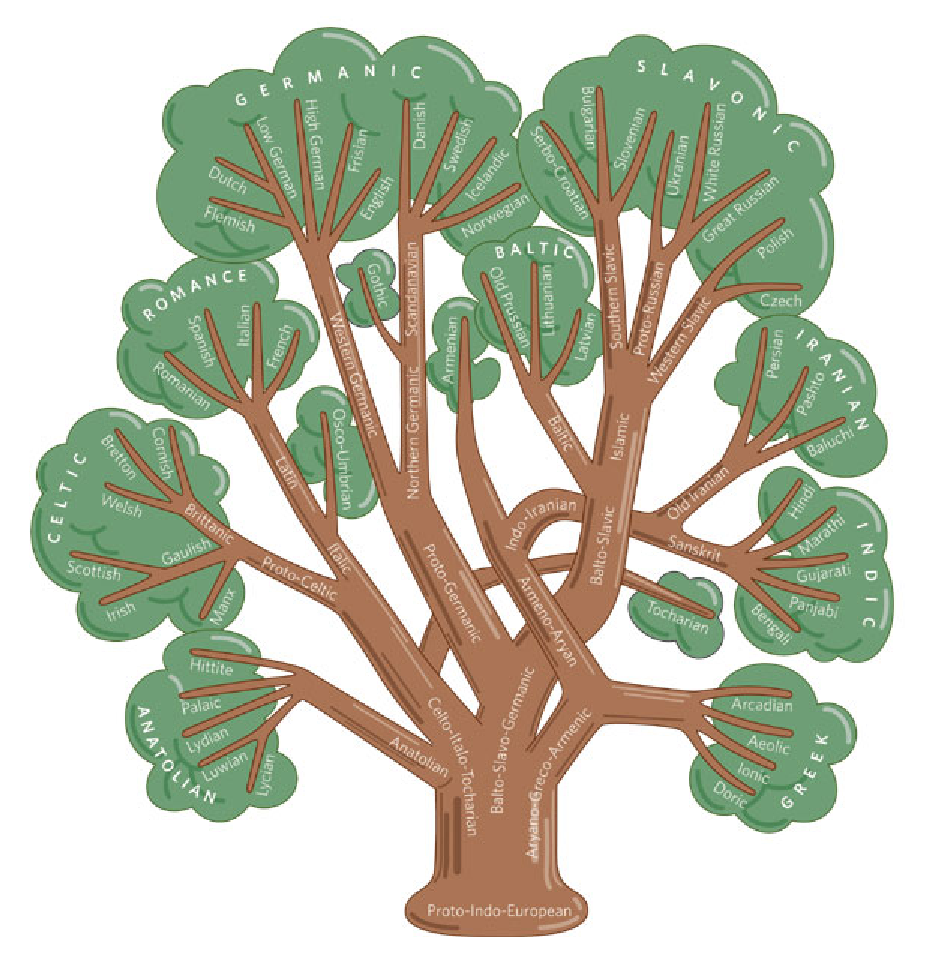
\includegraphics[width=\textwidth]{Pictures/indoeuropaeisch}
% \caption{\label{fig-indo-european-fitch}Language tree according to \citet[\page 665]{Fitch2007a-u}}
% \end{figure}
Proto-Germanic formed between 2000 and
1000 BCE. Its origins are in the Baltic region, that is, in northern Germany and southern
Scandinavia. About 500 BCE, the area where it was spoken extended from the North Sea to Poland.
The first written documents are runes from about 300 CE and the Gothic Bible translation in the fourth century.
The First Germanic Sound Shift took place before the second century BCE. In that millennium the
Germanic languages developed different consonants from the other Indo-European languages. 

Wikipedia\footnote{
\url{https://en.wikipedia.org/wiki/Germanic_languages}. 19.10.2014
} provides the table in Figure~\vref{fig-history-relations-germanic} that depicts the development of
the Germanic languages.
\begin{figure}
\begin{sideways}
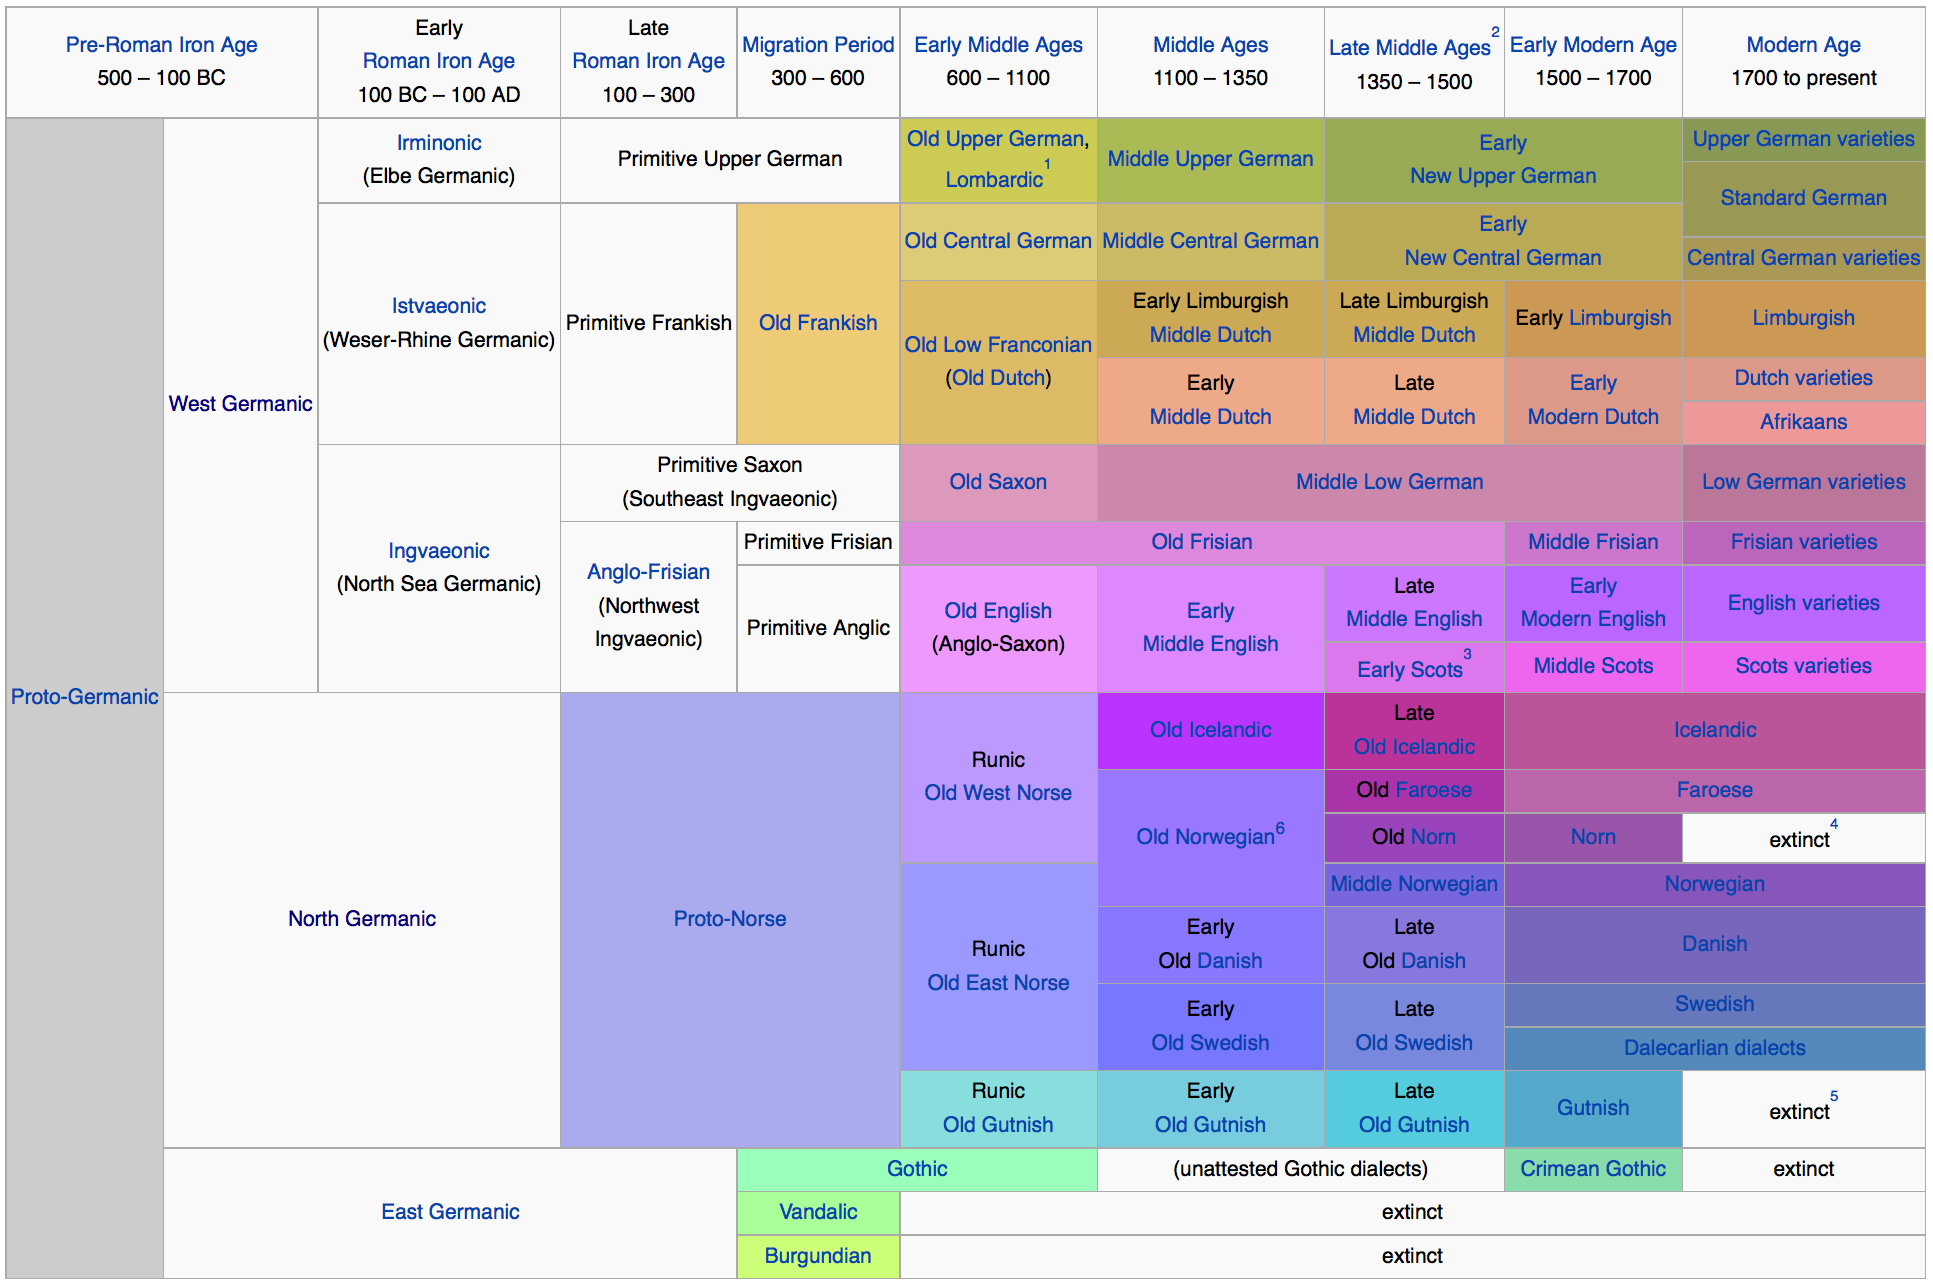
\includegraphics[width=.9\textheight]{Pictures/germanic-wikipedia}
\end{sideways}
\caption{\label{fig-history-relations-germanic}History and grouping of Germanic languages according to Wikipedia}
\end{figure}
Germanic is divided into East, West, and North Germanic. East Germanic existed in the form of Gothic
until about 1800 on the Crimea (Crimean Gothic) and is now totally extinct. 

West Germanic consists of 
\begin{itemize}
\item German, 
\item Yiddish, 
\item Luxembourgish, 
\item Pennsylvania Dutch, 
\item Low German, % Plattdeutsch or Niederdeutsch
\item Plautdietsch (also called Mennonite Low German), %
\item Dutch, 
\item Afrikaans, 
\item Frisian, and 
\item English.
\end{itemize}
The North Germanic languages are:
\begin{itemize}
\item Danish,
\item Swedish
\item Norwegian
\item Icelandic, and 
\item Faroese.
\end{itemize}


Table~\vref{tab-words-germanic} shows how similar the words from the main vocabulary of the Germanic
languages are:
\begin{table}
\centerfit{%
\begin{tabular}{lllllllll}
\hline\hline
Dutch & vader  & vier    & vol    & huis  & bruin  & uit & kruid     & muis\\
German        & Vater  & vier    & voll   & Haus  & braun  & aus & Kraut     & Maus\\
English       & father & four    & full   & house & brown  & out & crowd (?) & mouse\\
Frisian      & –      & fjouwer & fol    & hûs   & brún   & út  & krûd      & mûs\\
Swedish     & fader  & fyra    & full   & hus   & brun   & ut  & krut      & mus\\
Danish        & fader  & fire    & fuld   & hus   & brun   & ud  & krudt     & mus\\
Norwegian     & far    & fire    & full   & hus   & brun   & ut  & krydder   & mus\\
Iclandic     & faðir  & fjórir  & fullur & hús   & brúnn  & út  & –         & mús\\
\hline\hline
\end{tabular}
}
\caption{\label{tab-words-germanic}Words from the main vocabulary of some Germanic languages}
\end{table}

%% \section{Stammbaum der germanischen Sprachen}
%% 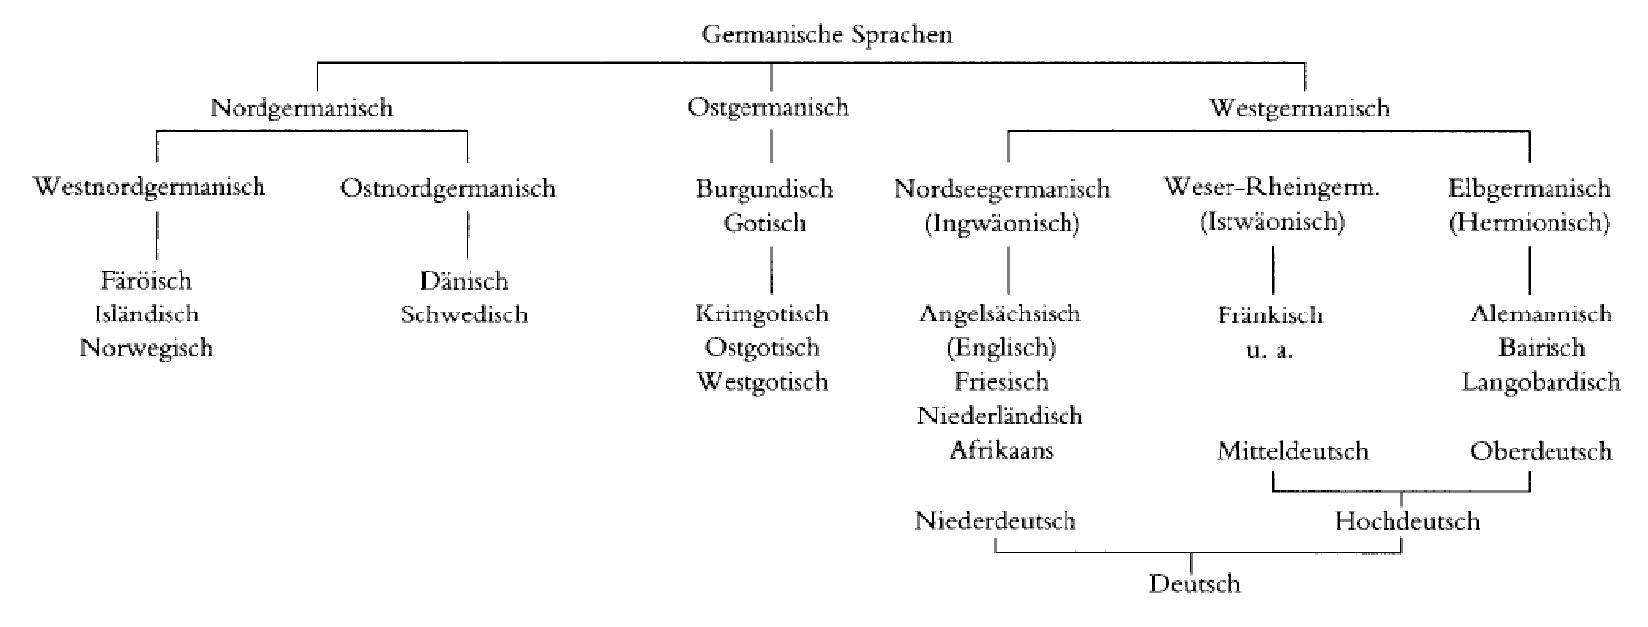
\includegraphics[width=\textwidth]{Pictures/stammbaum-germanisch}
%% aus \citew[S.\,251]{Bussmann2002a}





\section{The three branches of the Germanic family}

Proto-Germanic developed into the three main branches East, West, and North Germanic, approximately in
the first century CE. The reasons for this development were inherent variations in the respective
dialects, migration (language contact) and standardization. This book treats the structure of the
Germanic standard languages. This section is divided into three subsections that correspond to the
three main Germanic branches. I will sketch the historic developments that lead to the
languages spoken today. Many of the details that are covered in Figure~\ref{fig-history-relations-germanic} will be ignored.



\subsection{East Germanic}

The Goths emigrated from the Danish islands and South Sweden around 100 BCE and met the
Vandals and other tribes.  \ili{Gothic} and \ili{Burgundian} and some smaller languages constituted the East Germanic branch, of which only Gothic got passed on.
After the decay of the Gothic empires Gothic died out. There were some remains on the peninsula
Crimea until about 1800. The West Gothic bishop Wulfila translated the Bible into Gothic. The
best-known version of it is the fragment Codex Argenteus, which belongs to the university library of
Uppsala. Figure~\vref{fig-Wulfila-Bibel} shows a picture of it.\footnote{
Taken from Wikipedia: \url{http://de.wikipedia.org/wiki/Bild:Wulfila_bibel.jpg}. 19.10.2014.
}
\begin{figure}
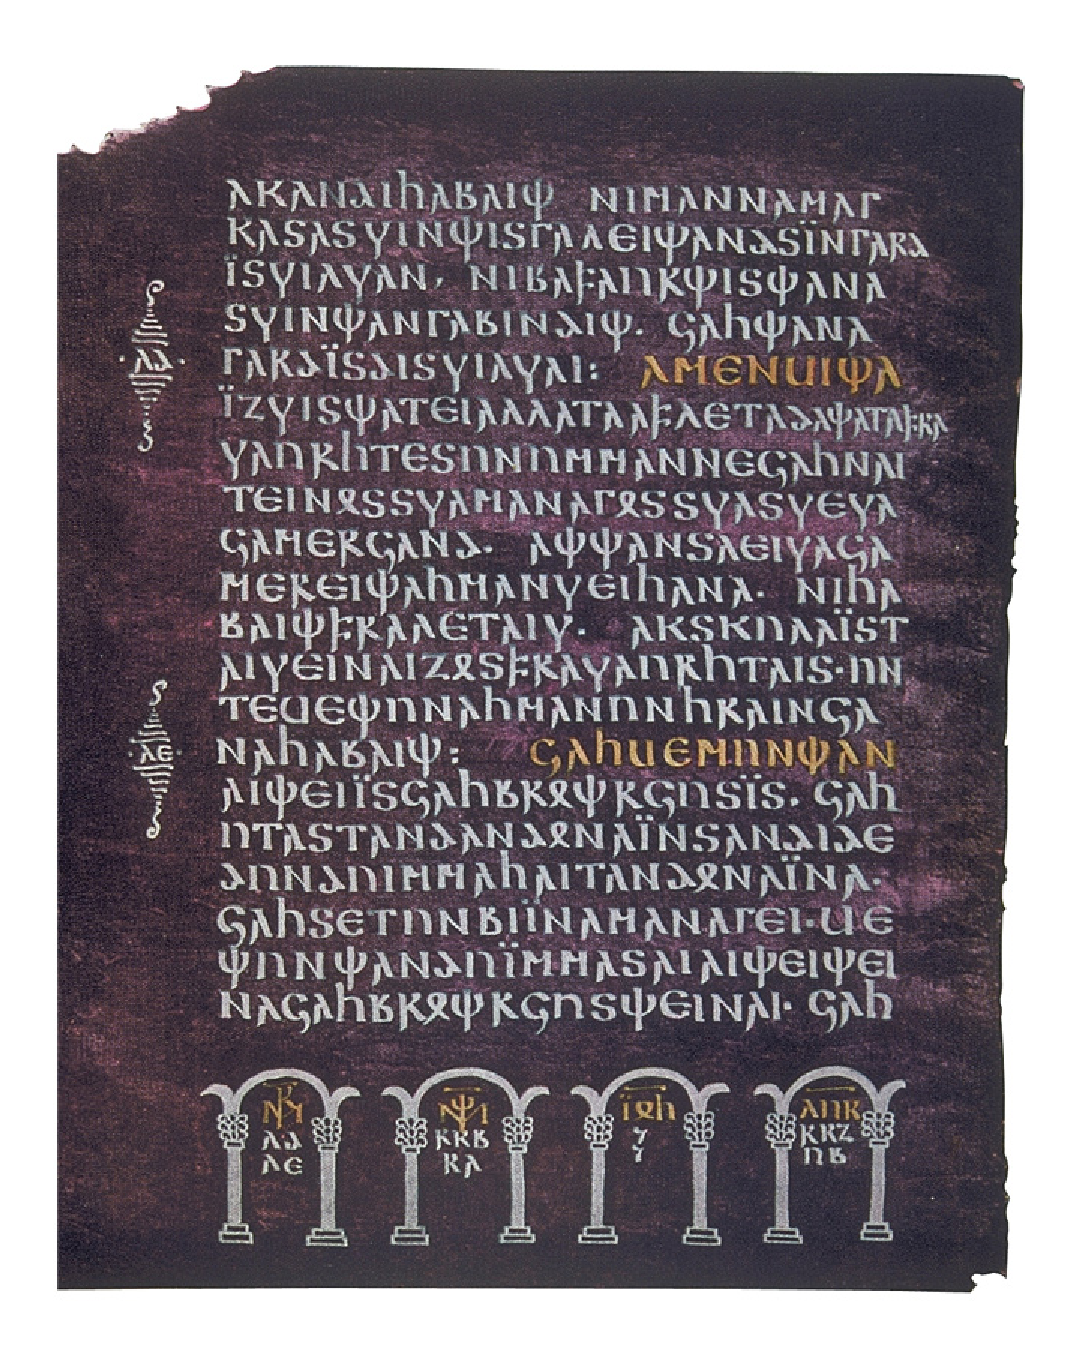
\includegraphics[width=53mm]{Pictures/Wulfila_bibel}
\caption{\label{fig-Wulfila-Bibel}The Wulfila Bible (Codex Argenteus), picture from Wikipedia}
\end{figure}



\subsection{North Germanic}

The first writings on runestones date back to the 6th century. The language of the Vikings
(800--1050) was rather homogeneous and it was only after this era that two branches were starting to
develop: the East-Scandinavian branch with Old-Danish and Old-Swedish and the West Scandinavian one
with Old-Norwegian and Old-Icelandic.


\subsubsection{Danish}

\ili{Danish} (dansk) is the official language of the
\href{https://en.wikipedia.org/wiki/Denmark}{Kingdom of Denmark} and the second official language of the
Faroe Islands and of Greenland, Inuit\il{Inuit} being the first official language of
Greenland. Danish has about 5,5 million speakers. About 50,000 speakers live in \href{https://en.wikipedia.org/wiki/Schleswig-Holstein}{Schleswig-Holstein}, the northernmost of the federal states of Germany.
Danish is the Scandinavian language that drifted furthest away from the common Scandinavian roots.


\subsubsection{Swedish}

\ili{Swedish} (svenska) is the official language in Sweden with about 8,5 million native speakers. It is
the first language of about 300,000 Swedish-speaking Finns in Finland. Until the times of the
Vikings Danish and Swedish were almost indistinguishable. Starting from about 800 they started to
diverge. Since about 1300 there are obvious differences.



\subsubsection{Icelandic}


\ili{Icelandic} (íslenska) is the West Scandinavian language of Iceland since its settlement over 1000 years ago. 
% Wikipedia 23.10.2014
There are about 325,000 native speakers. 97\,\% of the Icelandic population (325,000) has Icelandic as their
mother tongue and there are large groups of native speakers in Denmark, the USA, and Canada
(about 15,000 in total). 
There is less variation than in other Germanic languages (no dialects). 
%AZ that is too strong there is actually quite a bit of variation but maybe it is correct to say that there is less variation than in other Germanic languages
The language is conservative, in the sense that Icelandic
is the language among the Germanic languages that best preserved the Germanic vocabulary and inflection.
In the beginning there were almost no differences between Norwegian and Icelandic but
% The Dano-Norwegian, then later Danish rule of Iceland from 1536 to 1918 had little effect on the
% evolution of Icelandic (in contrast to the Norwegian language), which remained in daily use among
% the general population. 
% AZ: when?
starting about 1100 the languages diverged. This process continued also due to the Danish
influence and nowadays Norwegian is more similar to Danish than to Icelandic. There are many written documents in Icelandic.

\subsubsection{Norwegian}

There are two varieties of \ili{Norwegian} (norsk): Danish-Norwegian (bokmål) and New-Norwegian (nynorsk, landsmål). 
Both are official languages of Norway.
% and are used in parallel\itdopt{AZ: not clear what that means}. 
There are about 4,3 million speakers.
From 1380 to 1814 Danish was the written language and local dialects were spoken in Norway. It developed into the bokmål standard.
A standard that is less influenced by Danish was developed. This was done by Ivar Aasen (1813--1896), 
who developed Nynorsk. Nynorsk got an official status in 1885. Bokmål `book tongue' is the first language of most
of the Norwegians.

\subsubsection{Faroese}

\ili{Faroese} (føroyskt) is -- as well as Danish -- an official language of the Faroe Islands. There
are about 47,000 speakers. The Faroe Islands belong to Denmark since 1816. Since 1948 they are a
self-governing country within the \href{https://en.wikipedia.org/wiki/Danish_Realm}{Danish Realm}.
Faroese has a strong Danish influence. The first manuscript transmission is as recent as 1773 and
even after that date there are not many written documents. 
%AZ i would leave this out: (in contrast to Icelandic).And put something in the Icelandic section


\subsection{West Germanic}


Opinions on the question whether West Germanic developed from a single source or not differ. Some authors
assume that the West Germanic languages do not have a common root, but instead developed from the
following three unrelated branches of dialect groups (for instance \citealp[\page 17--18]{Robinson1992a-u} and
\citealp[\page 9]{HvDA94a}):
\begin{itemize}
\item North Sea Germanic %(Ingvaeonic, ancestral to Anglo-Frisian and also Old Saxon)
\item Weser-Rhine Germanic %(Istvaeonic, ancestral to Old Frankish, its successors Low Franconian and several dialects of Old High German)
\item Elbe Germanic %(Irminonic, ancestral to several dialects of Old High German, most probably including the extinct Langobardic language).
\end{itemize}
Other authors assume that these three branches had a common ancestor (see Figure~\ref{fig-history-relations-germanic}).

There is no unique mapping of these dialect groups to the languages spoken today.





\subsubsection{German}

\ili{German} is the official language of
\begin{itemize}
\item Germany (about 80 million speakers), 
\item Austria (about 7,5 million speakers), 
\item Liechtenstein (about 15,000 speakers), 
\item Switzerland (4,2 million of 6,4 million Swiss residents),
\item Northern Italy/South Tyrol (about 270,000 speakers), 
\item Belgium (about 65,000 speakers), and
\item Luxembourg (about 360,000 speakers).
\end{itemize}
Luxembourg has next to German also Luxembourgish and French as official
languages.

% There are about 97 million speakers of German, about, 90 of those are native speakers and 7 million
% have German as their second language.
% % = Migrationshintergrund
% % Quelle Wikipedia 15.10.2013
% Approximately 80 million speakers speak German as a foreign language, about 55 Million of these live
% in the European Union.%AZ It is a bit awkward to get these details for German but not for all the other languages

There are three main national variants (Germany, Austria, Switzerland). In other countries German is
%AZ leave out usually 
a minority language. There are two large dialect groups: Low German (Plattdüütsch,
Nedderdüütsch; in Standard German: Platt\-deutsch or Nie\-der\-deutsch%
%AZ this is clear as mud: do you
%want to say that Dutch is part of low Saxon or as most people do
%that low saxon are the dialects of German that are spoken in in the Netherlands? I would say:
%Nedersaksisch or Low Saxon, a group of dialects spoken in the Netherlands, southern Danmark and
%northwestern Germany
% Well, the areas in which Low Saxon is spoken overlap with national border. I speak about langauges
% spoken in these national borders here.
) and High German (varieties of German spoken south of the Benrath and Uerdingen
isoglosses).
%\itdopt{Stefan: fix}
%\todostefan{more}

% Wikipedia
%% The High German languages or High German dialects (German: Hochdeutsche Dialekte) comprise the varieties of German spoken south of the Benrath and Uerdingen isoglosses in central and southern Germany, Austria, Liechtenstein, Switzerland, and Luxembourg as well as in neighboring portions of Belgium (Eupen-Malmedy) and the Netherlands (Southeast Limburg), France (Alsace and northern Lorraine), Italy (South Tyrol), and Poland (Upper Silesia). They are also spoken in diaspora in Romania, Russia, the United States, Brazil, Argentina, Chile, and Namibia.

%% The High German languages are marked by the High German consonant shift, separating them from Low German and Low Franconian (Dutch) within the continental West Germanic dialect continuum.


%% Wikipedia

%% Middle Low German was the lingua franca of the Hanseatic League. It was the predominant language in Northern Germany. This changed in the 16th century: in 1534 the Luther Bible was published. This translation is considered to be an important step towards the evolution of the Early New High German. It aimed to be understandable to a broad audience and was based mainly on Central and Upper German varieties. The Early New High German language gained more prestige than Low German and became the language of science and literature. Around the same time, the Hanseatic league, based around northern ports, lost its importance as new trade routes to Asia and the Americas were established, while the most powerful German states of that period were located in Middle and Southern Germany.

%% The 18th and 19th centuries were marked by mass education in Standard German in schools. Gradually Low German came to be politically viewed as a mere dialect spoken by the uneducated. Today Low Saxon can be divided in two groups: Low Saxon varieties with a reasonable standard German influx[clarification needed] and varieties of Standard German with a Low Saxon influence known as Missingsch. Sometimes, Low Saxon and Low Franconian varieties are grouped together because both are unaffected by the High German consonant shift. However, the proportion of the population who can understand and speak it has decreased continuously since World War II.


%% Wikipedia
%% High German is divided into Central German, High Franconian (a transitional dialect), and Upper German. Central German dialects include Ripuarian, Moselle Franconian, Rhine Franconian, Central Hessian, East Hessian, North Hessian, Thuringian, Silesian German, Lorraine Franconian, Mittelalemannisch, North Upper Saxon, High Prussian, Lausitzisch-Neumärkisch and Upper Saxon. It is spoken in the southeastern Netherlands, eastern Belgium, Luxembourg, parts of France, and parts of Germany roughly between the River Main and the southern edge of the Lowlands. Modern Standard German is mostly based on Central German, although the common (but not linguistically correct) German term for modern Standard German is Hochdeutsch, that is, High German.

%% The Moselle Franconian varieties spoken in Luxembourg have been officially standardised and institutionalised and are usually considered a separate language known as Luxembourgish.

%% The two High Franconian dialects are East Franconian and South Franconian.

%% Upper German dialects include Northern Austro-Bavarian, Central Austro-Bavarian, Southern Austro-Bavarian, Swabian, East Franconian, High Alemannic German, Highest Alemannic German, Alsatian and Low Alemannic German. They are spoken in parts of the Alsace, southern Germany, Liechtenstein, Austria, and the German-speaking parts of Switzerland and Italy.

%% Wymysorys is a High German dialect of Poland native to Wilamowice, and Sathmarisch and Siebenbürgisch are High German dialects of Romania. The High German varieties spoken by Ashkenazi Jews (mostly in the former Russian Empire) have several unique features, and are usually considered as a separate language, Yiddish. It is the only Germanic language that does not use the Latin script as the basis of its standard alphabet.


\subsubsection{Yiddish}

\ili{Yiddish} is one of many languages spoken in the Jewish diaspora. About 2 million people speak this language in various
regions of the world, most of them in the USA (1,25 Mill.). The number of Yiddish speakers was much
higher 100 years ago: 7 million speakers of Yiddish lived in Europe, most of them in Russia and in
Austria-Hungary. At most 75,000 Yiddish speakers are left in Western Europe. Yiddish has its roots
in medieval German with influences from \ili{Hebrew} and \ili{Aramaic}.




\subsubsection{Pennsylvania German}

\ili{Pennsylvania German} (Pensilfaanish, Deitsch), which is also known as Pennsylvanian Dutch has about 300,000
native speakers, who mainly live in the USA. The most important regions are Pennsylvania, Ohio, and
Indiana. Pennsylvania German is the result of immigration in the 17th and 18th century. Members of
various protestant religions (Mennonites, Pietists and so on) left Europe for religious reasons  
but later immigrants that came for economic reasons followed.  The language is
based on Palatine dialects and is nowadays mainly spoken by Amish and Mennonites.




\subsubsection{Dutch}

\ili{Dutch} (Nederlands) is the  official language of the Netherlands and has about 15 million speakers in that country. Dutch is also one of the official languages of Belgium with about 6 million speakers.
%AZleave out: ; almost 4 million Walloones). 
Dutch is the sole official language and teaching language in Suriname, 
%AZ leave out: which is independent since 1975, 
% 60% of the population speak it as their mother tongue % wikipedia
% 24% speak it as a second language
and in \href{https://en.wikipedia.org/wiki/Aruba}{Aruba} and the \href{https://en.wikipedia.org/wiki/Netherlands_Antilles}{Netherlands Antilles}.

%In Aruba, Curaçao and Sint Maarten, all parts of the Kingdom of the Netherlands, Dutch is the official language but spoken as a first language by only 7% to 8% of the population,[56] although most native-born people on the islands can speak the language since the education system is in Dutch at some or all levels.[57] The lingua franca of Aruba, Bonaire and Curaçao is Papiamento, a creole language that originally developed among the slave population. The population of the three northern Antilles, Sint Maarten, Saba, and Sint Eustatius, is predominantly English-speaking.[44]

\subsubsection{Afrikaans}

\ili{Afrikaans} is one of the official languages of South Africa since 1925, which has eleven official languages.
There are about 6,4 million native speakers in South Africa, which is about 15\,\% of the population,
and 150,000 in Namibia. Afrikaans developed since the 17th century from \ili{Dutch} dialects and is seen
as an independent language since somewhere between 1775 and 1850 \citep{denBesten2012a-u}.
% Oft wird gesagt, dass ab ca. 1775 von 'Afrikaans' gesprochen werden kann (Den Besten spricht aber noch vom 'Proto-Afrikaans'). Die Übergänge vom Kap-Niederländischen zum Afrikaans sind natürlich fließend, aber um die Zeit herum, gibt es doch schon genügend dokumentierte Unterschiede, um zu sagen, dass Afrikaans eine eigenständige Sprache geworden ist. Allerspätestens ab Mitte des 19. Jahhunderts ist dann aber auf jeden Fall eine eigene Sprache anzusetzen; da sind sich alle einig. Und 1925 wird das dann ja auch offizielle Amtssprache. 
The various African languages spoken in the area interacted with Afrikaans.
%AZ leave out: and its origins and resulted in a structural simplification in comparison to Dutch
Today English has a strong influence.



\subsubsection{Frisian}

The three varieties of \ili{Frisian} are mutually not intelligible. There is North Frisian spoken by
about 10,000 speakers mainly on the north Frisian islands Amrum, Sylt, and Helgoland. East Frisian
is extinct with the exception of Saterlandic, which is spoken in the three villages of Saterland
(Landkreis Cloppenburg) by between 1,000 and 2,500 people.
% https://www.taz.de/!5834717 Inseln
West Frisian is spoken in the northern Dutch province Fryslân (Friesland) and has about 350,000
native speakers.



\subsubsection{English}

All over the world \ili{English} had about 570 million speakers at the end of the 20th century 
(337 million native speakers, 235 million speakers with English as the second language\footnote{%
  The term \emph{Zweitsprache} `second language' is used to refer to speakers using a language in
  everyday life since there surrounding uses this language. An example would be speakers with
  Turkish as their first language living in Germany. The German tradition distinguishes
  \emph{Zweitsprache} from \emph{Fremdsprache} `foreign language'.%
}). The countries with the most native speakers are listed below: 
\begin{itemize}
\item USA: 227 million,
\item Great Britain: 57 million,
\item Nigeria: 43 million, 
\item Canada: 24 million,
\item Australia: 17 million,
\item Ireland: 3,5 million,
\item New Zealand: 3,2 million.
\end{itemize}
There are many national variants, which differ mostly in pronunciation.
Between 1 and 1,5 billion people have active or passive knowledge of English.
English is an official language in 59 states. It is the most important scientific language.




%      <!-- Local IspellDict: en_US-w_accents -->
